\subsection{Backend}

\begin{figure*}
	\centering
	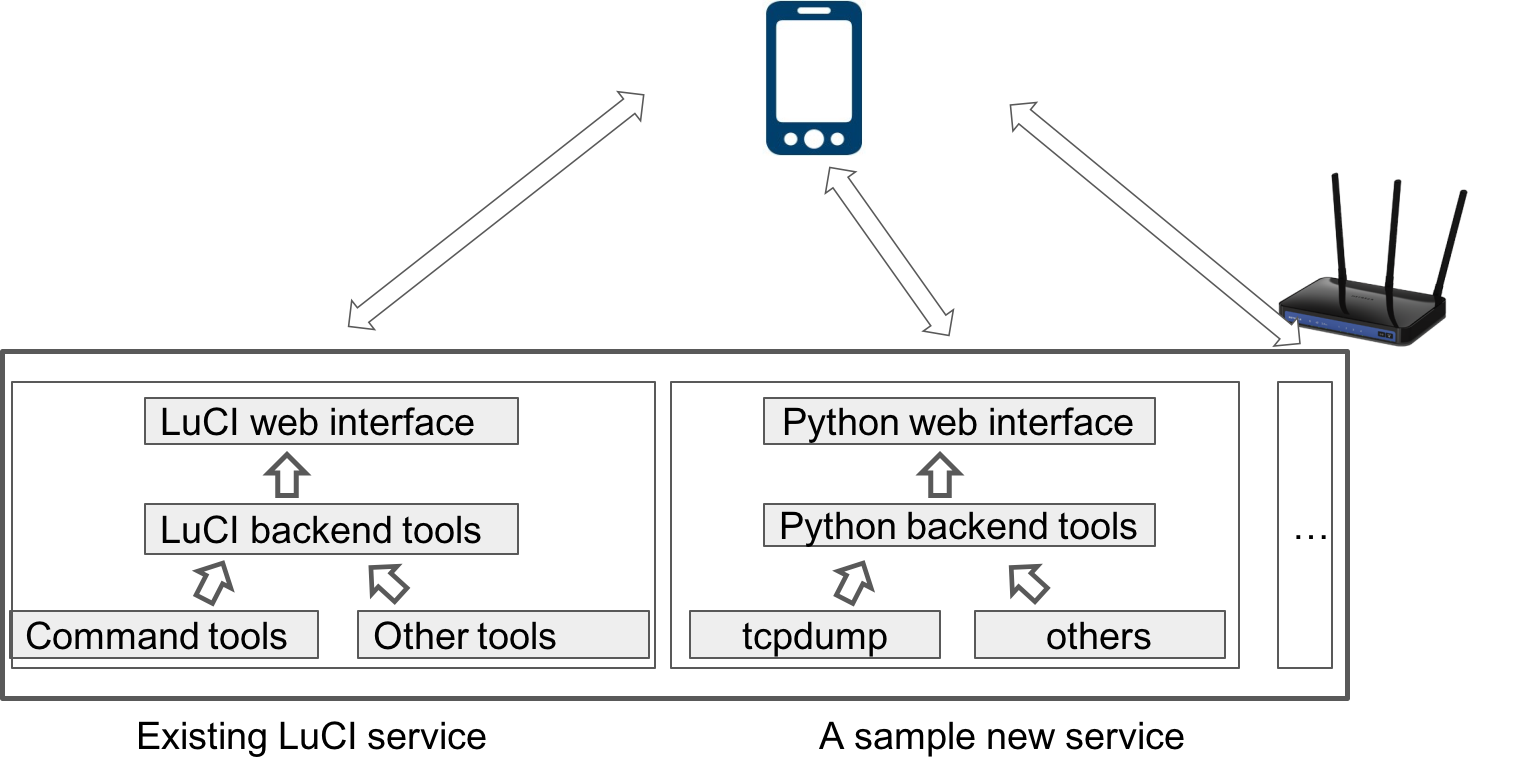
\includegraphics[width=0.75\textwidth]{backend-architecture.png}
	\caption{Backend Architecture}
	\label{backend-architecture}
\end{figure*}

This sub-section describes the design of the system backend. For basic configuration functions, we decide to reuse (and extend) services from LuCI, a mature configuration web service running on OpenWRT, since LuCI backend provides most of the functions needed to monitor network status and configure networks. However, the per-device per-application network usage statistics is not gathered by LuCI. To provide extra functions such as this one, we decide to build an additional Python service on OpenWRT. Figure \ref{backend-architecture} shows the architecture of the backend.

\subsubsection{LuCI web service/interface}

LuCI backend provides useful tools to operate OpenWrt. For example, ``luci.sys'' package can be used to call system functions, ``'luci.http'' package can be used to deal with http protocols, ``luci.controller.rpc'' can be used to call remote processes, and ``luci.util.exec'' can be used to execute shell commands. LuCI provides an http interface to access its backend, which covers enough functionalities for our application's purposes, such as monitoring system load, and configuring WiFi interface.

\subsubsection{Per-application statistics analysis}
\label{sec:app-specific-design}

One of the goals in this project was to identify and provide statistics for traffic belonging to specific user applications, such as quantifying incoming and outgoing traffic related to specific smartphone application and services, and determining the identities of the hosts generating the traffic going through the OpenWRT box. To achieve this goal, we considered the two following design approaches:

\textbf{(A).} Pre-install a service on each user device that would monitor application network usage information from the operating system and report the monitored statistics to a service on the OpenWRT box. This approach can likely generate very accurate results and provide each specific application's statistical network usage. However, the major drawback to this method of collecting accurate traffic information is that it requires that each user voluntarily install and run this service on their devices, a requirement non-ideal for our goal: this service should not require additional actions and permissions from user devices, and the OpenWRT box should be able to collect statistics with or without end user cooperation.
	
\textbf{(B).}  Capture the traffic on the OpenWRT box, and run per-packet analysis. While less accurate than the first option, it is less intrusive to the user. The following information components from packet headers or payloads could be used to capture and analyze traffic:
	
\begin{itemize}
	
	\item Source and destination IP addresses. 
	
	Popular service providers, such as Google and Facebook, own large chunks of IP addresses, and certain IP address ranges may correspond to servers for a specific application. By collecting such information and building a  mapping from destination IP address to an application's backend services, it is possible to infer which user application generated the traffic. The problem with this approach is that this mapping takes time to build, and dynamically changing the mapping in response to newly collected information is difficult, especially considering the fact that many popular services are using CDNs.
	
	\item Source and destination port number. 
	
	Certain services can be identified by IANA's port number allocation \cite{touch2013service}, and this information is easily retrievable from the Internet. The problem with this approach is that the number of applications that can be identified purely by port number is very limited, as some applications will share the same ports. For example, the Youtube and Facebook apps on Android both go through port 443 (TLS).
	
	\item Application layer payload. 
	
	Decoding application payload and trying to find characteristic plain text is another way to identify which application a packet belongs to. This approach is promising, except it works only if such characteristic texts can be located and the application payload has not encrypted, which is not the case for most popular Android applications, such as Youtube or Facebook. Packet capturing of these Android applications shows that their traffic goes on top of TLS \cite{dierks2008transport}, and packet capturing of the activity of watching Youtube videos on a desktop indicates that the traffic goes on top of QUIC \cite{QUIC}, which has encryption over UDP.
	
	\item Source and destination host names. 
	
	DNS host names often give information about the service provider, even when the service provider's using CDNs. By doing a DNS reverse lookup \cite{eidnes1998classless} on the IP addresses, we can find out the service's domain name, thus infer what application's generating the traffic. The assumption behind this approach is that most servers or CDN boxes have a DNS name that corresponds to the application backend that they run. Our initial experiments suggest that this assumption is indeed true for popular applications like Youtube and Facebook, though mapping a DNS domain to a certain service may not be straightforward. For example, Facebook app on Android talks to both \textit{*.facebook.com} domain, and \textit{*.fbcdn.net} (owned by the CDN provider, Akamai Technologies) domain, and Youtube app talks to both \textit{*.google.com}, and \textit{*.1e100.net}, another Google owned domain. 
	
	Given this caveat, the authors chose the last approach since it is most applicable than other options listed above. For the proof-of-concept implementation, the mapping from domain names to service names is statically configured. It is also worth mentioning that this approach will limit our statistics to per service provider, rather than per exact application (for example, the traffic application is unable to differentiate Google Hangout application traffic from Youtube application traffic), but the authors believe this approach is enough for the purpose of providing statistics on the router end that provides a network adminstrator a reasonable amount of information to determine which applications on which devices are generating how much traffic.

\end{itemize} 
	
Table \ref{appfilterchoice} summarizes the above approaches.

\begin{table*}
	\centering
	\caption{Traffic Analysis Approaches}
	\label{appfilterchoice}
	\begin{tabular}{p{4cm}|p{2cm}|p{10cm}} \hline
		Analysis Approaches & Work or not? & Reason \\ \hline
		IP addresses & No & Popular apps (such as Youtube, Facebook) use different servers to distribute contents, we cannot know the mapping between IP addresses and applications \\ \hline
		TCP ports & No & TCP ports are not assigned for specific apps\\ \hline
		Application payload & No  & Popular apps (such as Youtube, Facebook) use TLS\\ \hline
		DNS Domain name & Yes & Use nslookup to map IP addresses to domain names first. And then map domain names to applications \\
		\hline\end{tabular}
\end{table*}